\documentclass[cn,11pt,chinese]{elegantbook}

\usepackage[all]{xy}
\usepackage{amsmath}
\usepackage{asymptote}
\usepackage{subfig}
\usepackage{graphicx}



\newcount\mycount
\def\cis{\,\text{cis}\,}
\def\intset{\operatorname{int}}
\def\diam{\operatorname{diam}}
\def\dist{\operatorname{dist}}
\def\ulim{\operatorname{u-lim}}
\def\cinfty{\mathbb{C}_{\infty}}
\def\sh{\operatorname{sh}}
\def\argsh{\operatorname{argsh}}
\def\ch{\operatorname{ch}}
\def\argch{\operatorname{argch}}
\def\real{\mathbb{R}}
\def\dsint{{\displaystyle\int}}

\numberwithin{equation}{section}


% title info
\title{抽象代数}

% bio info
\author{Dummit D. S. and Foote R.M.}

% extra info
\version{1.00}
\extrainfo{Wir m\"ussen wissen, wir werden wissen. (我们必须知道,我们必将知道) - David.Hilbert}
%\logo{logo.png}
\cover{cover.jpg}

\begin{document}


\maketitle

\tableofcontents
\mainmatter
\hypersetup{pageanchor=true}

\chapter*{Preface}
\addcontentsline{toc}{chapter}{Preface}
This book evolved out of notes by the authors from courses given at various universities over a period of about thirteen years. The backgrounds of students in these courses were 


\chapter*{Preliminaries}\label{chapter000}
\addcontentsline{toc}{chapter}{Preliminaries}
Some results and notation that are used throughout the text are collected in this chapter for convenience. Students may wish to review this chapter quickly at first and then read each section more carefully again as the concepts appear in the course of the text.

\section{Basics}\label{section00001}
The basics of set theory: sets, $\cap$, $\cup$, $\in$, etc. should be familiar to the reader. Our notation for subsets of a given set $A$ will be
\[
B = \{a \in A | \cdots (\text{conditions on a}) \cdots\}.
\]
The order or cardinality of a set $A$ will be denoted by $|A|$. If $A$ is a finite set the order of $A$ is simply the number of elements of $A$.

It is important to understand how to test whether a particular $x \in A$ lies in a subset $B$ of $A$ (cf. Exercises 1 to 4). The Cartesian product of two sets $A$ and $B$ is the collection $A \times B = \{(a, b)| a \in A, b \in B\}$, of ordered pairs of elements from $A$ and $B$.

We shall use the following notation for some common sets of numbers:
\begin{enumerate}
\item[(1)] $\mathbb{Z}= \{0, \pm{1}, \pm{2}, \pm{3}\cdots\}$ denotes the integers (the $\mathbb{Z}$ is for the German word for numbers: "Zahlen").
\item[(2)] $\mathbb{Q} = \{a/b|a, b \in \mathbb{Z}, b \neq 0\}$ denotes the rational numbers (or rationals).
\item[(3)] $\real = \{\text{all decimal expansions }\pm{d_1d_2\cdots d_n.a_1a_2a_3\cdots}\}$ denotes the real numbers (or reals).
\item[(4)] $\mathbb{C} = \{a + bi|a, b \in \real, i^2 = -1\}$ denotes the complex numbers.
\item[(5)] $\mathbb{Z}^+$, $\mathbb{Q}^+$ and $\real^+$ will denote the positive (nonzero) elements in $\mathbb{Z}$, $\mathbb{Q}$ and $\real$, respectively.
\end{enumerate}

We shall use the notation $f: A \to B$ or $A \stackrel{f}{\rightarrow} B$ to denote a function $f$ from $a$ to $B$ and the value of $f$ at $a$ is denoted $f(a)$ (i.e. we shall apply our functions on the left). We use the words function and map interchangeably. The set $A$ is called the domain of $f$ and $B$ is called the codomain of $f$. The notation $f: a \mapsto b$ or $a \mapsto b$ if $f$ is understood indicates that $f(a)=b$, i.e. the function is being specified on elements.

If the function $f$ is not specified on elements it is important in general to check that $f$ is well defined, i.e. is unambiguously determined. For example, if the set $A$ is the union of two subsets $A_1$ and $A_2$ then one can try to specify a function from $A$ to the set $\{0, 1\}$ by declaring that $f$ is to map everything in $A_1$ to 0 and is to map everything in $A_2$ to 1. This unabiguously defines $f$ unless $A_1$ and $A_2$ have elements in common (in which case it is not clear whether these elements should map to 0 or to 1). Checking that this $f$ is well defined therefore amounts to checking that $A_1$ and $A_2$ have no intersection.

The set
\[
f(A) = \{b \in B | b = f(a), \text{for some } a \in A\}
\]
is a subset of $B$, called the range or image of $f$ (or the image of $A$ under $f$). For each subset $C$ of $B$ the set
\[
f^{-1}(C) = \{a \in A | f(a) \in C\}
\]
consisting of the elements of $A$ mapping into $C$ under $f$ is called the preimage or inverse image of $C$ under $f$. For each $b \in B$, the preimage of $\{b\}$ under $f$ is called the fiber of $f$ over $b$. Note that $f^{-1}$ is not in general a function and that the fibers of $f$ generally contain many elements since there may be many elements of $A$ mapping to the element $b$.

If $f:A \to B$ and $g: B \to C$, then the composite map $g \circ f: A \to C$ is defined by
\[
(g \circ f)(a) = g(f(a)).
\]

Let $f:A \to B$.
\begin{enumerate}
\item[(1)] $f$ is injective or is an injection if whenever $a_1 \neq a_2$, then $f(a_1) \neq f(a_2)$.

\item[(2)] $f$ is surjective or is a surjection if for all $b \in B$ there is some $a \in A$ such that $f(a) = b$, i.e. the image of $f$ is all of $B$. Note that since a function always maps onto its range (by definition) it is necessary to specify the codomain $B$ in order for the question of surjectivity to be meaningful.

\item[(3)] $f$ is bijective or is a bijection if it is both injective and surjective, If such a bijection $f$ exists from $A$ to $B$, we say $A$ and $B$ are in bijective correspondence.

\item[(4)] $f$ has a left inverse if there is a function $g:B \to A$ such that $g \circ f:A \to A$ is the identity map on $A$, i.e. $(g \circ f)(a)=a$, for all $a \in A$.

\item[(5)] $f$ has a right inverse if there is a function $h:B \to A$ such that $f \circ h:B \to B$ is the identity map on $B$.
\end{enumerate}

\begin{proposition}{}{prop0000101}
Let $f:A \to B$.
\begin{enumerate}
\item[(1)] The map $f$ is injective if and only if $f$ has a left inverse.
\item[(2)] The map $f$ is surjective if and only if $f$ has a right inverse.
\item[(3)] The map $f$ is bijective if and only if there exists $g:B \to A$ such that $f \circ g$ is the identity map on $B$ and $g \circ f$ is the identity map on $A$.
\item[(4)] If $A$ and $B$ are finite sets with the same number of elements (i.e. $|A|=|B|$). then $f:A \to B$ is bijective if and only if $f$ is injective if and only if $f$ is surjective.
\end{enumerate}
\end{proposition}

\begin{proof}
Exercise.
\end{proof}

In the situation fo part (3) of the proposition above the map $g$ is necessarily unique and we shall say $g$ is the 2-sided iverse (or simply the inverse) of $f$.

A permutation of a set $A$ is simply a bijection from $A$ to itself.

If $A \subset B$ and $f: B \to C$, we denote the restriction of $f$ to $A$ by $f|_A$. When the domain we are  considering is understood we shall occasionally denote $f|_A$ again simply as $f$ even though these are formally different functions (their domains are different).

If $A \subset B$ and $g: A \to C$ and there is a function $f: B \to C$ such that $f|_A = g$, we shall say $f$ is an extension of $g$ to $B$ (such a map $f$ need not exist nor be unique).

Let $A$ be a nonempty set.
\begin{enumerate}
\item[(1)] A binary relation on a set $A$ is a subset $R$ of $A \times A$ and we write $a \sim b$ if $(a, b)\in R$.
\item[(2)] The relation $\sim$ on $A$ is said to be: 
\begin{enumerate}
\item[(a)] reflexive if $a \sim a$, for all $a \in A$,
\item[(b)] symmetric if $a \sim b$ implies $b \sim a$ for all $a, b \in A$,
\item[(c)] transitive if $a \sim b$ and $b \sim c$ implies $a \sim c$ for all $a,b,c \in A$.
\end{enumerate}
A relation is an equivalence relation if it is reflexive, symmetric and transitive.

\item[(3)] If $\sim$ defined an equivalence relation on $A$, then the equivalence class of $a \in A$ is defined to be $\{x \in A| x \sim a\}$. Elements of the equivalence class of $a$ are said to be equivalent to $a$. If $C$ is an equivalence class, any element of $C$ is called a representative of the class $C$.

\item[(4)] A partition of $A$ is any collection $\{A_i|i\in I\}$ of nonempty subsets of $A$ ($I$ some indexing set) such that
\begin{enumerate}
\item[(a)] $A = \cup_{i \in I}{A_i}$, and
\item[(b)] $A_i \cap A_j = \emptyset$, for all $i, j \in I$ with $i \neq j$.
\end{enumerate}
i.e. $A$ is the disjoint union of the sets in the partition.
\end{enumerate}

The notions of an equivalence relation on $A$ and a partition of $A$ are the same:

\begin{proposition}{}{prop0000102}
Let $A$ be an nonempty set.
\begin{enumerate}
\item[(1)]  If $\sim$ defines an equivalece relation on $A$ then the set of equivalence classes of $\sim$ form a partition of $A$.
\item[(2)] If $\{A_i | i \in I\}$ is a partition of $A$ then there is an eqivalence relation on $A$ whose equivalence classes are precisely the sets $A_i$, $i \in I$.
\end{enumerate}
\end{proposition}

\begin{proof}
Omitted.
\end{proof}

Finally, we shall assume the reader is familiar with proofs by induction.

In Exercises 1 to 4 let $\mathcal{A}$ be the set of $2 \times 2$ matrices with real numbers entries. Recall that matrix multiplication is defined by
\[
\begin{pmatrix}a & b\\ c & d\end{pmatrix}\begin{pmatrix}p & q\\r & s\end{pmatrix}=
\begin{pmatrix}ap+br & aq + bs\\cp+dr& cq + ds\end{pmatrix}
\]
Let
\[
M = \begin{pmatrix}1 & 1 \\0 & 1\end{pmatrix}
\]
and let 
\[
\mathcal{B} = \{X \in \mathcal{A} | MX = XM\}.
\]

\begin{problemset}
\item Determine which of the following elements of $\mathcal{A}$ lie in $\mathcal{B}$:
\begin{gather*}
\begin{pmatrix}
1 & 1\\
0 & 1
\end{pmatrix},
\begin{pmatrix}
1 & 1\\
1 & 1
\end{pmatrix},
\begin{pmatrix}
0 & 0\\
0 & 0
\end{pmatrix},
\begin{pmatrix}
1 & 1\\
1 & 0
\end{pmatrix},
\begin{pmatrix}
1 & 0\\
0 & 1
\end{pmatrix},
\begin{pmatrix}
0 & 1\\
1 & 0
\end{pmatrix}.
\end{gather*}

\item Prove that if $P, Q \in \mathcal{B}$, then $P+Q\in \mathcal{B}$ (where $+$ denotes the usual sum of two matrices).

\item Prove that if $P, Q \in \mathcal{B}$, then $P\cdot Q \in \mathcal{B}$ (where $\cdot$ denotes the usual product of two matrices).

\item Find conditions on $p, q, r, s$ which determine precisely when $\begin{pmatrix}p & q \\r & s\end{pmatrix} \in \mathcal{B}$.

\item Determine whether the following functions $f$ are well defined:
\begin{enumerate}
\item[(a)] $f:\mathbb{Q} \to \mathbb{Z}$ defined by $f(a/b) = a$.
\item[(b)] $f:\mathbb{Q} \to \mathbb{Q}$ defined by $f(a/b) = a^2/b^2$.
\end{enumerate}

\item Determine whether the function $f:\real^+ \to \mathbb{Z}$ defined by mapping a real number $r$ to the first digit to the right of the decimal point in a decimal expansion of $r$ is well defined.

\item Let $f: A \to B$ be a surjective map of sets. Prove that the relation
\[
a \sim b \text{ if and only if } f(a) = f(b)
\]
is an equivalence relation whose equivalence classes are the fibers of $f$.

\end{problemset}



\section{Properties of the integers}\label{section00002}
The following properties of the integers $\mathbb{Z}$ (many familiar from elementary arithmetic) will be proved in a more general context in the ring theory of Chapter \ref{chapter008}, but it will be necessary to use them in Part I (of course, none of the ring theory proofs of these properties will rely on the group theory).

\begin{enumerate}
\item[(1)] (Well Ordering of $\mathbb{Z}$) If $A$ is any nonempty subset of $\mathbb{Z}^+$, there is some element $m \in A$ such that $m \le a$, for all $a \in A$ ($m$ is called a minimal element of $A$).

\item[(2)] If $a, b \in \mathbb{Z}$ with $a \neq 0$, we say $a$ divides $b$ if there is an element $c \in \mathbb{Z}$ such that $b=ac$. In this case we write $a \mid b$; if $a$ does not divide $b$ we write $a \nmid b$.

\item[(3)] If $a, b \in \mathbb{Z} - \{0\}$, there is a unique positive integer $d$, called the greatest common divisor of $a$ and $b$ (or g.c.d.  of $a$ and $b$), satisfying:
\begin{enumerate}
\item[(a)] $d \mid a$ and $d \mid b$ (so $d$ is a common divisor of $a$ and $b$), and
\item[(b)] if $e \mid a$ and $e \mid b$, then $e \mid d$ (so $d$ is the greatest such divisor).
\end{enumerate}
The g.c.d. of $a$ and $b$ will be denoted by $(a, b)$. If $(a, b) = 1$, we say that $a$ and $b$ are relatively prime.

\item[(4)] If $a, b \in \mathbb{Z} - \{0\}$, there is q unique positive integer $l$, called least common multiple of $a$ and $b$ (or l.e.m. of $a$ and $b$), satisfying:
\begin{enumerate}
\item[(a)] $a \mid l$ and $b \mid l$ (so $l$ is a common multiple of $a$ and $b$), and
\item[(b)] if $a \mid m$ and $b \mid m$, then $l \mid m$ (so $l$ is the least such multiple).
\end{enumerate}
The connection between the greatest common divisor $d$ and the least common multiple $l$ of two integers $a$ and $b$ is given by $dl=ab$.

\item[(5)] The Division Algorithm: if $a, b \in \mathbb{Z} -\{0\}$, then there exist unique $q, r\in \mathbb{Z}$ such that
\[
a = qb + r \quad \text{and} \quad 0 \le r < |b|,
\]
where $q$ is the quotient and $r$ the remainder, This is the usual "long division" familiar from elementary arithmetic.

\item[(6)] The Euclidean Algorithm is an important procedure which produces a greatest common divisor of two integers $a$ and $b$ by iterating the Division Algorithm: if $a, b \in \mathbb{Z} - \{0\}$, then we obtain a sequence of quotients and remainders
\begin{gather}
a = q_0b + r_0 \tag{0}\\
b = q_1r_0 + r_1 \tag{1}\\
r_0 = q_2r_1 + r_2 \tag{2}\\
r_1 = q_3r_2 + r_3 \tag{3}\\
\vdots \notag\\
r_{n-2} = q_nr_{n-1} + r_n \tag{n}\\
r_{n-1} = q_{n+1}r_n \tag{n+1}
\end{gather}
where $r_n$ is the last nonzero remainder. Such an $r_n$ exists since $|b| > |r_0| > |r_1| > \cdots > |r_n|$ is a decreasing sequence of strictly positive integers if the remainders are nonzero and such a sequence cannot continue indefinitely. Then $r_n$ is the g.c.d. (a, b) of $a$ and $b$.

\begin{example}
Suppose $a = 57970$ and $b=10353$. Then applying the Euclidean Algorithm we obtain:
\[
\begin{aligned}
57970 &= (5)10353 + 6205\\
10353 &= (1)6205 + 4148\\
6205 &= (1)4148 + 2057\\
4148 &= (2)2057 + 34\\
2057 &= (60)34 + 17\\
34 &= (2)17
\end{aligned}
\]
which shows that $(57970, 10353) = 17$.
\end{example}

\item[(7)] One consequence of the Euclidean Algorithm which we shall use regularly is the following: if $a, b, \in \mathbb{Z} - \{0\}$, then there exist $x, y \in \mathbb{Z}$ such that
\[
(a, b) = ax + by
\]
that is, the g.c.d. of $a$ and $b$ is a $\mathbb{Z}$-linear combination of $a$ and $b$. This follows by recursively writing the element $r_n$ in the Euclidean Algorithm in terms of the previous remainders (namely, use equation (n) above to solve for $r_n = r_{n-2} - q_nr_{n-1}$ in terms of the remainders $r_{n-1}$ and $r_{n-2}$, then use equation (n-1) to write $r_n$ in terms of the remainders $r_{n-2}$ and $r_{n-3}$, etc. eventually writing $r_n$ in terms of $a$ and $b$).

\begin{example}
Suppose $a = 57970$ and $b=10353$, whose greatest common divisor we computed above to be 17. From the fifth equation (the next to last equation) in the Euclidean Algorithm applied to these two integers we solve for their greatest common divisor: $17 = 2057 - (60)34$. The fourth equation then shows that $34 = 4148 - (2)2057$, so substituting this expression for the previous remainder 34 gives the equation $17 = 2057 - (60)[4148 - (2)2057]$, i.e. $17 = (121)2057 - (60)4148$. Solving the third equation for 2057 and substituting gives $17 = (121)[6205 - (1)4148] - (60)4148 = (121)6205 - (181)4148$. Using the second equation to solve for 4148 and then the first equation to solve for 6205 we finally obtain
\[
17 = (302)57970 - (1691)10353
\]
as can easily be checked directly. Hence the equation $ax + by = (a, b)$ for the geatest common divisor of $a$ and $b$ in this example has the solution $x = 302$ and $y=-1691$. Note that it is relatively unlikely that this relation would have been found simply by guessing.
\end{example}

The integers $x$ and $y$ in (7) above are not unique. In the example with $a = 57970$ and $b = 10353$ we determined one solution to be $x = 302$ and $y = -1691$, for instance, and it is relatively simple to check that $x = -307$ and $y = 1719$ also satisfy $57970x + 10353y=17$. The general solution for $x$ and $y$ is known (cf. the exercises below and in Chapter \ref{chapter008}).

\item[(8)] An element $p$ of $\mathbb{Z}^+$ is called a prime if $p > 1$ and the only positive divisors of $p$ are 1 and $p$ (initially, the word prime will refer only to positive integers). An integer $n > 1$ which is not prime is called composite. For example, $2,3,5,7,11,13,17,19, \cdots$ are primes and $4,6,8,9,12,14,15,16,18, \cdots$ are composite.

An important property of primes (which in fact can be used to define the primes (cf. Exercise 3)) is the following: if $p$ is a prime and $p \mid ab$, for some $a, b \in \mathbb{Z}$, then either $p \mid a$ or $p \mid b$.

\item[(9)] The Fundamental Theorem of Arithmetic says: if $n \in \mathbb{Z}$, $n > 1$, then $n$ can be factored uniquely into the product of primes, i.e. there are distinct primes $p_1, p_2, \cdots, p_s$ and positive integers $\alpha_1, \alpha_2, \cdots, \alpha_s$ such that
\[
n = p_1^{\alpha_1}p_2^{\alpha_2}\cdots{}p_s^{\alpha_s},
\]
This factorization is unique in the sense that if $q_1, q_2, \cdots, q_t$ are any distinct primes and $\beta_1, \beta_2, \cdots, \beta_t$ positive integers such that
\[
n = q_1^{\beta_1}q_2^{\beta_2}\cdots{}q_t^{\beta_t},
\]
then $s=t$ and if we arrange the two sets of primes in increasing order, then $q_i = p_i$ and $\alpha_i = \beta_i$, $1 \le i \le s$. For example, $n = 1852423848 = 2^33^211^219^331$ and this decomposition into the product of primes is unique.

Suppose the positive integers $a$ and $b$ are expressed as products of prime powers:
\[
a = p_1^{\alpha_1}p_2^{\alpha_2} \cdots p_s^{\alpha_s}, \quad b = p_1^{\beta_1}p_2^{\beta_2}\cdots p_s^{\beta_s}
\]
where $p_1,p_2,\cdots,p_s$ are distinct and the exponents are $\ge 0$ (we allow the exponents to be 0 here so that the products are taken over the same set of primes - the exponent will be 0 if that prime is not actually a divisor). Then the greatest common divisor of $a$ and $b$ is
\[
(a, b) = p_1^{\min(\alpha_1, \beta_1)}p_2^{\min(\alpha_2, \beta_2)}\cdots{}p_s^{\min(\alpha_s, \beta_s)}
\]
(and the least common multiple is obtained by instead taking the maximum of the $\alpha_i$ and $\beta_i$ instead of the minimum).

\begin{example}
In the example above, $a = 57970$ and $b = 10353$ can be factored as $a = 2 \cdot 5 \cdot 11 \cdot 17 \cdot 31$ and $b = 3 \cdot 7 \cdot 17 \cdot 29$, from which we can immediately conclude that their greatest common divisor is 17. Note, however, that for large integers it is extremely difficult to determine their prime factorizations (several common codes in current use are based on this difficulty, in fact), so that this is not an effective method to determine greatest common divisor in general. The Euclidean Algorithm will produce greatest common divisors quite rapidly without the need for the prime factorization of $a$ and $b$.
\end{example}

\item[(10)] The Euler $\varphi-$function is defined as follows: for $n \in \mathbb{Z}^+$ let $\varphi(n)$ be the number of positive integers $a \le n$ with $a$ relatively prime to $n$, i.e. $(a, n) = 1$. For example, $\varphi(12) = 4$ since $1,5,7$ and $11$ are the only positive integers less than or equal to 12 which have no factors in common with 12. Similarly, $\varphi(1)=1$, $\varphi(2)=1$, $\varphi(3)=2$, $\varphi(4)=2$, $\varphi(5)=4$, $\varphi(6)=2$, etc. For primes $p$, $\varphi(p) = p - 1$, nd, more generally, for all $a \ge 1$ we have the formula
\[
\varphi(p^{\alpha}) = p^{\alpha} - p^{\alpha-1} = p^{\alpha-1}(p-1).
\]
The function $\varphi$ is \emph{multiplication} in the sense that 
\[
\varphi(ab) = \varphi(a)\varphi(b)\quad \text{if }(a, b) = 1
\]
(note that it is important here that $a$ and $b$ be relatively prime). Together with the formula above this gives a general formula for the values of $\varphi$: if $n = p_1^{\alpha_1}p_2^{\alpha_2}\cdots{}p_s^{\alpha_s}$, then
\[
\begin{aligned}
\varphi(n) &= \varphi(p_1^{\alpha_1})\varphi(p_2^{\alpha_2})\cdots\varphi(p_s^{\alpha_s})\\
&=p_1^{\alpha_1-1}(p_1-1)p_2^{\alpha_2-2}(p_2-1)\cdots{}p_s^{\alpha_s-1}(p_s-1).
\end{aligned}
\]
For example, $\varphi(12) = \varphi(2^2)\varphi(3)=2^1(2-1)3^0(3-1)=4$. The reader should note that we shall use the letter $\varphi$ for many different functions throughout the text so we want this letter to denote Euler's function we shall be careful to indicate this explicitly.


\end{enumerate}

\begin{problemset}
\item For each of the following pairs of integers $a$ and $b$, determine their greatest common divisor, their least common multiple, and write their greatest common divisor on the form $ax + by$ for some integers $x$ and $y$.
\begin{enumerate}
\item[(a)] $a = 20$, $b = 13$.
\item[(b)] $a = 69$, $b = 372$.
\item[(c)] $a = 792$, $b = 275$.
\item[(d)] $a = 11391$, $b = 5673$.
\item[(e)] $a = 1761$, $b = 1567$.
\item[(f)] $a = 507885$, $b = 60808$.
\end{enumerate}

\item Prove that if the integer $k$ divides the integers $a$ and $b$ then $k$ divides $as + bt$ for every pair of integers $s$ and $t$.

\item Prove that if $n$ is composite then there are integers $a$ and $b$ such that $n$ divides $ab$ but $n$ does not divide either $a$ or $b$.

\item Let $a$, $b$ and $N$ be fixed integers with $a$ and $b$ nonzero and let $d = (a, b)$ be the greatest common divisor of $a$ and $b$. Suppose $x_0$ and $y_0$ are particular solutions to $ax + by = N$ (i.e. $ax_0 + by_0 = N$). Prove for any integer $t$ that the integers
\[
x = x_0 + \frac{b}{d}t \quad\text{and}\quad y = y_0 - \frac{a}{d}t
\]
are also solutions to $ax + by = N$ (this is in fact the general solution).

\item Determine the value $\varphi(n)$ for each integer $n \le 30$ where $\varphi$ denotes the Euler $\varphi-$function.

\item Prove the Well Ordering Property of $\mathbb{Z}$ by induction and prove the minimal element is unique.

\item If $p$ is a prime prove that there do not exist nonzero integers $a$ and $b$ such that $a^2 = pb^2$(i.e. $\sqrt{p}$ is not a rational number).

\item Let $p$ be a prime, $n \in \mathbb{Z}^+$. Find a formular for the largest power of $p$ which divides $n!=n(n-1)(n-2)\cdots{}2\cdot{}1$ (it involves the greatest integer function).

\item Write a computer program to determine the greatest common divisor $(a, b)$ of two integers $a$ and $b$ and to express $(a, b)$ in the form $ax + by$ for some integers $x$ and $y$.

\item Prove for any given positive integer $N$ there exist only finitely many integers $n$ with $\varphi(n) = N$ where $\varphi$ denotes Euler's $\varphi-$function. Conclude in particular that $\varphi(n)$ tends to infinity as $n$ tends to infinity.

\item Prove that if $d$ divides $n$ then $\varphi(d)$ divides $\varphi(n)$ where $\varphi$ denotes Euler's $\varphi-$function.

\end{problemset}


\section{$\mathbb{Z}/n\mathbb{Z}$: The integers Modulo $n$}\label{section00003}
Let $n$ be a fixed positive integer. Define a relation on $\mathbb{Z}$ by
\[
a \sim b \text{ if and only if }n \mid (b - a).
\]
Clearly $a \sim a$, and $a \sim b$ implies $b \sim a$ for any integers $a$ and $b$, so this relation is trivially reflexive and symmetric. If $a \sim b$ and $b \sim c$ then $n$ divides $a-b$ and $n$ divides $b-c$ so $n$ also divides the sum of these two integers, i.e. $n$ divides $(a-b) + (b-c) = a-c$, so $a \sim c$ and the relation is transitive. Hence this is an equivalence relation. Write $a \equiv b \pmod{n}$ (read: $a$ is congruent to $b \bmod{n}$) if $a \sim b$. For any $k \in \mathbb{Z}$ we shall denote the equivalence class of $a$ by $\bar{a}$ - this is called the congruence class or residue class of $a \bmod{n}$ and consists of the integers which differ from $a$ by an integeral multiple of $n$, i.e.
\[
\begin{aligned}
\bar{a} &= \{ a + kn | k \in \mathbb{Z}\}\\
&= \{a, a \pm n, a \pm{2n}, a \pm{3n},\cdots\}.
\end{aligned}
\]
There are precisely $n$ distinct equivalence classes $\bmod{n}$, namely
\[
\bar{0}, \bar{1}, \bar{2}, \cdots, \overline{n-1}
\]
determined by the possible remainders after division by $n$ and these residue classes partition the integers $\mathbb{Z}$. The set of equivalence classes under this equivalence relation  will be denoted by $\mathbb{Z}/n\mathbb{Z}$ and called the integers modulo $n$ (or the integers $\bmod{n}$). The motivation for this notation will become clearer when we discuss quotient groups and quotient rings. Note that for different $n$'s the equivalence relation and equivalence classes are different so we shall always be careful to fix $n$ first before using the bar notation. The process of finding the equivalence class $\bmod{n}$ of some integer $a$ is often referred to as reducing $a \bmod{n}$. This terminology also frequently refers to finding the smallest nonnegative integer congruent to $a \bmod{n}$ (the least residue of $a \bmod{n}$).

We can define an addition and a multiplication for the elements of $\mathbb{Z}/n\mathbb{Z}$, defining modular arithmetic as follows: for $\bar{a}, \bar{b} \in \mathbb{Z}/n\mathbb{Z}$, define their sum and product by
\[
\bar{a} + \bar{b} = \overline{a + b} \quad\text{and}\quad \bar{a} \cdot \bar{b} = \overline{ab}.
\]
What this means is the following: given any two elements $\bar{a}$ and $\bar{b}$ in $\mathbb{Z}/n\mathbb{Z}$, to compute their sum (respectively, their product) take any representative integer $a$ in the class $\bar{a}$ and any representative integer $b$ in the class $\bar{b}$ and add (respectively, multiply) the integers $a$ and $b$ as usual in $\mathbb{Z}$ and then take the equivalence class containing the result. The following Theorem 3 asserts that this is well defined, i.e. does not depend on the choice of representatives taken for the elements $\bar{a}$ and $\bar{b}$ of $\mathbb{Z}/n\mathbb{Z}$.

\begin{example}
Suppose $n=12$ and consider $\mathbb{Z}/12\mathbb{Z}$, which consists of the twelve residue classes
\[
\bar{0},\bar{1},\bar{2},\cdots,\overline{11}
\]
determined by the twelve possible remainders of an integer after division by 12. The elements in the residue class $\bar{5}$, for example, are the integers which leave a remainder of 5 when divided by 12 (the integers congruent to 5 $\bmod{12}$). Any integer congruent to 5 $\bmod{12}$ (such as $5,17, 29, \cdots$ or $-7, -19, \cdots$) will serve as a representative for the residue class $\bar{5}$. Note that $\mathbb{Z}/12\mathbb{Z}$ consists of the twelve elements above (and each of these elements of $\mathbb{Z}/12\mathbb{Z}$ consists of an infinite number of usual integers).

Suppose now that $\bar{a}=\bar{5}$ and $\bar{b} = \bar{8}$. The most obvious representative for $\bar{a}$ is the integer 5 and similarly 8 is the most obvious representative for $\bar{b}$. Using these representatives for the residue classes we obtain $\bar{5} = \bar{8} = \overline{13} = \bar{1}$ since 13 and 1 lie in the same class modulo $n=12$. Had we instead taken the representative 17, say, for $\bar{a}$ (note that 5 and 17 do lie in the same residue class modulo 12) and the representative $-28$, say, for $\bar{b}$, we would obtain $\bar{5} + \bar{8} = \overline{17 - 28} = \overline{-11} = \bar{1}$ and as we mentioned the result does not depend on the choice of representatives chosen. The product of these two classes is $\bar{a} \cdot \bar{b} = \overline{5 \cdot 8} = \overline{40} = \bar{4}$, also independent of the representatives chosen.
\end{example}

\begin{theorem}{}{thm0000303}
The operations of addition and multiplication on $\mathbb{Z}/n\mathbb{Z}$ defined above are both well defined, that is, they do not depend on the choices of representatives for the classes involved. More precisely, if $a_1, a_2 \in \mathbb{Z}$ and $b_1, b_2 \in \mathbb{Z}$ with $\overline{a_1} = \overline{b_1}$ and $\overline{a_2} = \overline{b_2}$, then $\overline{a_1 + a_2} = \overline{b_1+b_2}$ and $\overline{a_1a_2} = \overline{b_1b_2}$. i.e. if
\[
a_1 \equiv b_1 \pmod{n} \quad \text{and}\quad a_2 \equiv b_2 \pmod{n}
\]
then
\[
a_1 + a_2 \equiv b_1 + b_2 \pmod{n} \quad \text{and}\quad a_1a_2 \equiv b_1b_2 \pmod{n}
\]
\end{theorem}

\begin{proof}
Suppose $a_1 \equiv b_1\pmod{n}$, i.e. $a_1-b_1$ is divisible by $n$. Then $a_1 = b_1 + sn$ for some integer $s$. Similarly, $a_2\equiv b_2\pmod{n}$ means $a_2 = b_2 + tn$ for some integer $t$. Then $a_1+a_2 = (b_1+b_2) + (s+t)n$ so that $a_1+a_2 \equiv b_1+b_2 \pmod{n}$, which shows that the sum of the residue classes is independent of the representatives chosen. Similarly, $a_1a_2 = (b_1+sn)(b_2+tn) = b_1b_2 + (b_1t + b_2s + st)n$ shows that $a_1a_2 \equiv b_1b_2 \pmod{n}$ and so the product of the residue classes is also independent of the representatives chosen, completing the proof.
\end{proof}

We shall see later that the process of adding equivalence classes by adding their representatives is a special case of a more general construction (the construction of a quotient). This notion of adding equivalence classes is already a familiar one in the context of adding rational numbers: each rational number $a/b$ is really a class of expressions: $a/b = 2a/2b = -3a/-3b$ etc. and we often change representatives (for instance, take common denominators) in order to add two fractions (for example $1/2 + 1/3$ is computed by taking instead the equivalent representatives $3/6$ for $1/2$ and $2/6$ for $1/3$ to obtain $1/2+1/3=3/6+2/6=5/6$). The notion of modular arithmetic is also familiar: to find the hour of day after adding or subtracting some number of hours we reduce $\bmod{12}$ and find the least residue.

It is important to be able to think of the equivalence classes of some equivalence relation as elements which can be manipulated (as we do, for example, with fractions) rather than as sets. Consistent with this attitude, we shall frequently denote the elements of $\mathbb{Z}/n\mathbb{Z}$ simply by $\{0,1, \cdots, n-1\}$ where addition and multiplication are reduced $\bmod{n}$. It is important to remember, however, that the elements of $\mathbb{Z}/n\mathbb{Z}$ are not integers, but rather collections of usual integers, and the arithmetic is quite different. For example, $5 + 8$ is not 1 in the integers $\mathbb{Z}$ as it was in the example of $\mathbb{Z}/12\mathbb{Z}$ above.

The fact that one can define arithmetic in $\mathbb{Z}/n\mathbb{Z}$ has many important applications in elementary number theory. As one simply example we compute the last two digits in the  number $2^{1000}$. First observe that the last two digits give the remainder of $2^{1000}$ after we divide by 100 so we are interested in the residue class $\bmod{100}$ containing $2^{1000}$. We compute $2^{10} = 1024 \equiv 24 \pmod{100}$, so then $2^{20} = (2^{10})^2 \equiv 24^2 = 576 \equiv 76 \pmod{100}$. Then $2^{40} = (2^{20})^2  \equiv 76^2 = 5776 \equiv 76 \pmod{100}$. Similarly $2^{80} \equiv 2^{160} \equiv 2^{320} \equiv 2^{640} \equiv 76 \pmod{100}$. Finally, $2^{1000} = 2^{640}2^{320}2^{40} \equiv 76 \cdot 76 \cdot 76 \equiv 76 \pmod{100}$ so the final two digits are 76.

An important subset $\mathbb{Z}/n\mathbb{Z}$ consists of the collection of residue classes which have a multiplicative inverse in $\mathbb{Z}/n\mathbb{Z}$:
\[
(\mathbb{Z}/n\mathbb{Z})^{\times} = \{\bar{a} \in \mathbb{Z}/n\mathbb{Z} | \text{there exists }\bar{c} \in \mathbb{Z}/n\mathbb{Z} \text{ with } \bar{a} \cdot \bar{c} =\bar{1}\}.
\]
Some of the following exercises outline a proof that $(\mathbb{Z}/n\mathbb{Z})^{\times}$ is also the collection of residue classes whose representatives are relatively prime to $n$:
\begin{proposition}{}{prop0000304}
$(\mathbb{Z}/n\mathbb{Z})^{\times} = \{\bar{a} \in \mathbb{Z}/n\mathbb{Z} | (a, n) = 1\}$.
\end{proposition}

It is easy to see that if any representative of $\bar{a}$ is relatively prime to $n$ then all representatives are relatively prime to $n$ so that the set on the right in the proposition is well defined.

\begin{example}
For $n=9$ we obtain $(\mathbb{Z}/9\mathbb{Z})^{\times} = \{1,2,4,5,7,8\}$ from the proposition. The multiplicative inverses of these elements are $\{1, 5, 7, 2, 4, 8\}$, respectively.
\end{example}

If $a$ is an integer relatively prime to $n$ then the Euclidean Algorithm produces integers $x$ and $y$ satisfying $ax + ny = 1$, hence $ax \equiv 1 \pmod{n}$, so that $\bar{x}$ is the multiplicative inverse of $\bar{a}$ in $\mathbb{Z}/n\mathbb{Z}$. This gives an efficient method for computing multiplicative inverses in $\mathbb{Z}/n\mathbb{Z}$.

\begin{example}
Suppose $n = 60$ and $a = 17$. Applying the Euclidean Algorithm we obtain
\[
\begin{aligned}
60 &= (3)17 + 9\\
17 &= (1)9 + 8\\
9 &= (1)8 + 1
\end{aligned}
\]
so that $a$ and $n$ are relatively prime, and $(-7)17 + (2)60 = 1$. Hence $\overline{-1} = \overline{53}$ is the multiplicative inverse of $\overline{17}$ in $\mathbb{Z}/60\mathbb{Z}$.
\end{example}

\begin{problemset}
\item Write down explicitly all the elements in the residue classes of $\mathbb{Z}/18\mathbb{Z}$.

\item Prove that the distinct equivalence classes in $\mathbb{Z}/n\mathbb{Z}$ are precisely $\bar{0}, \bar{1}, \bar{2}, \cdots, \overline{n-1}$(use the Division Algorithm).

\item Prove that if $a= a_n10^n + a_{n-1}10^{n-1} + \cdots + a_110 + a_0$ is any positive integer then $a \equiv a_n + a_{n-1} + \cdots +a_1+a_0 \pmod{9}$ (note that this is the usual arithmetic rule that the remainder after division by 9 is the same as the sum of the decimal digits $\bmod{9}$ - in particular an integer is divisible by 9 if and only if the sum of its digits is divisible by 9)[note that $10 \equiv 1\pmod{9}$].

\item Compute the remainder when $37^{100}$ is divided by 29.

\item Compute the last two digits of $9^{1500}$.


\end{problemset}

% add preface chapter here if needed
\part{Group Theory}
\chapter{Introduction to Groups}\label{chapter001}
\section{Basic Axioms and Examples}\label{section00101}


\section{Dihedral Groups}\label{section00102}



\section{Symmetric Groups}\label{section00103}



\section{Matrix Groups}\label{section00104}



\section{The Quaternion Groups}\label{section00105}



\section{Homomorphisms and Isomorphisms}\label{section00106}



\section{Group Actions}\label{section00107}




\chapter{Subgroups}\label{chapter002}
\section{Definition and Examples}\label{section00201}


\chapter{Euclidean Domains, Principal Ideal Domains and Unique Factorization Domains}\label{chapter008}





% \bibliographystyle{plain}
\bibliography{mathreference}
\appendix
% h
\chapter{Tikz绘制的一些图形}
\begin{center}
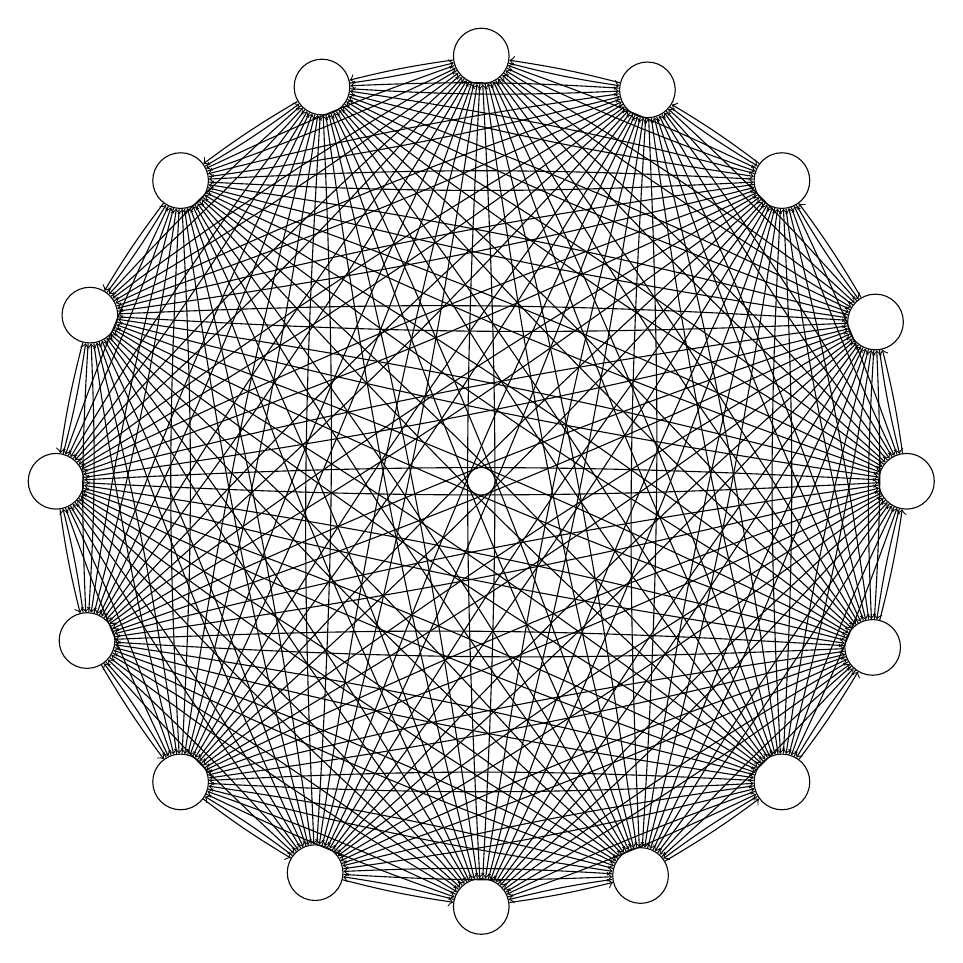
\begin{tikzpicture}[transform shape]
  %the multiplication with floats is not possible. Thus I split the loop in two.
  \foreach \number in {1,...,8}{
      % Computer angle:
        \mycount=\number
        \advance\mycount by -1
  \multiply\mycount by 45
        \advance\mycount by 0
      \node[draw,circle,inner sep=0.25cm] (N-\number) at (\the\mycount:5.4cm) {};
    }
  \foreach \number in {9,...,16}{
      % Computer angle:
        \mycount=\number
        \advance\mycount by -1
  \multiply\mycount by 45
        \advance\mycount by 22.5
      \node[draw,circle,inner sep=0.25cm] (N-\number) at (\the\mycount:5.4cm) {};
    }
  \foreach \number in {1,...,15}{
        \mycount=\number
        \advance\mycount by 1
  \foreach \numbera in {\the\mycount,...,16}{
    \path (N-\number) edge[->,bend right=3] (N-\numbera)  edge[<-,bend
      left=3] (N-\numbera);
  }
}
\end{tikzpicture}


\begin{tikzpicture}
 \definecolor{r1}{RGB}{0,129,188}
 \definecolor{r2}{RGB}{252,177,49}
 \definecolor{r3}{RGB}{35,34,35}
 \definecolor{r4}{RGB}{0,157,87}
 \definecolor{r5}{RGB}{238,50,78}
 \begin{scope}
   \clip (-6,2) rectangle (6,-.9);
   \foreach \col/\xp/\yp in {
     r5/4/0, r4/2/-1.8, r3/0/0,
     r2/-2/-1.8, r1/-4/0
   } {
     \path[draw=white,line width=.08cm,
     fill=\col,even odd rule]
     (\xp, \yp) circle (1.9cm)
     (\xp, \yp) circle (1.5cm);
   }
 \end{scope}
 \begin{scope}
   \clip (-6,-.9) rectangle (6,-3.8);
   \foreach \col/\xp/\yp in {
     r1/-4/0, r2/-2/-1.8, r3/0/0,
     r4/2/-1.8, r5/4/0
   } {
     \path[draw=white,line width=.08cm,
     fill=\col,even odd rule]
     (\xp, \yp) circle (1.9cm)
     (\xp, \yp) circle (1.5cm);
   }
 \end{scope}
\end{tikzpicture}


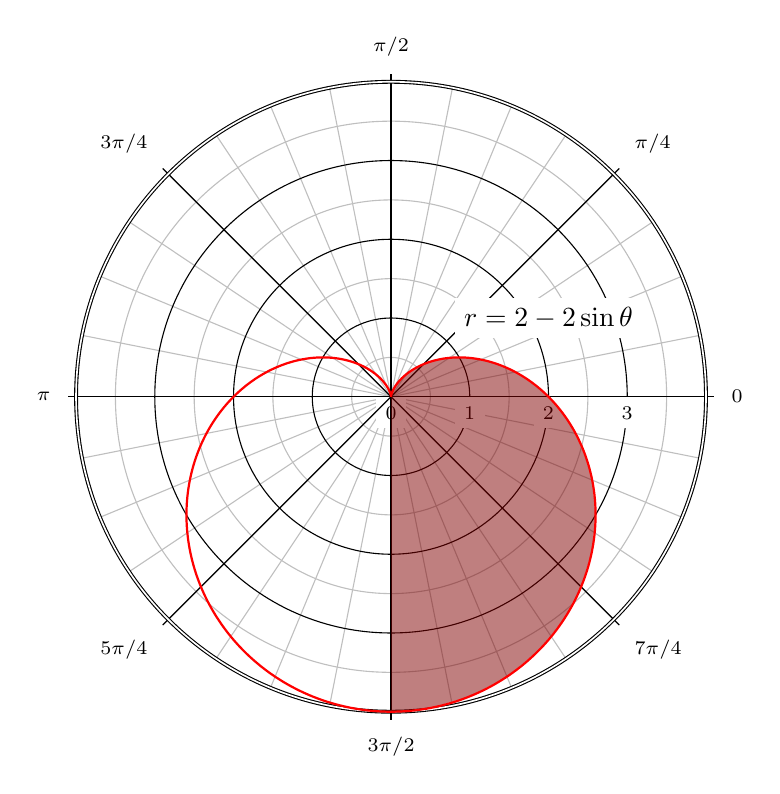
\begin{tikzpicture}[>=latex]

% Draw the lines at multiples of pi/12
\foreach \ang in {0,...,31} {
  \draw [lightgray] (0,0) -- (\ang * 180 / 16:4);
}

% Concentric circles and radius labels
\foreach \s in {0, 1, 2, 3} {
  \draw [lightgray] (0,0) circle (\s + 0.5);
  \draw (0,0) circle (\s);
  \node [fill=white] at (\s, 0) [below] {\scriptsize $\s$};
}

% Add the labels at multiples of pi/4
\foreach \ang/\lab/\dir in {
  0/0/right,
  1/{\pi/4}/{above right},
  2/{\pi/2}/above,
  3/{3\pi/4}/{above left},
  4/{\pi}/left,
  5/{5\pi/4}/{below left},
  7/{7\pi/4}/{below right},
  6/{3\pi/2}/below} {
  \draw (0,0) -- (\ang * 180 / 4:4.1);
  \node [fill=white] at (\ang * 180 / 4:4.2) [\dir] {\scriptsize $\lab$};
}

% The double-lined circle around the whole diagram
\draw [style=double] (0,0) circle (4);

\fill [fill=red!50!black, opacity=0.5] plot [domain=-pi/2:pi/2]
  (xy polar cs:angle=\x r, radius= {2-2*sin(\x r)});
\draw [thick, color=red, domain=0:2*pi, samples=200, smooth]
  plot (xy polar cs:angle=\x r, radius={2-2*sin(\x r)});
\node [fill=white] at (2,1) {$r=2-2\sin\theta$};

\end{tikzpicture} 


% definition de partial ellipse
\tikzset{partial ellipse/.style args =
  {#1:#2:#3}{insert path={+ (#1:#3) arc (#1:#2:#3)}}}
\begin{tikzpicture}[>=latex]
  %  ellipses
  \draw [fill=white!90!red]    (3,-1.8) ellipse    (4cm and 1 cm);
  \draw [fill=yellow!90!green] (3,-1.8) ellipse (3cm and 0.75 cm);
  \draw [fill=white!90!green]  (3,-1.8) ellipse  (2cm and 0.5 cm);

  % -- Soleil
  \shade [ball color=gray!10!yellow] (3,-1.8) circle (1);
  \node (soleil) at (3,-1.8) {\bf Soleil};
  % partial ellipse pour tracé devant le Soleil
  \draw (3,-1.8) [partial ellipse=220:320:2cm and 0.5cm]
        (3,-1.8) [partial ellipse=220:320:3cm and 0.75cm];

  % Venus
  \shade [ball color=gray!10!orange] (1.6,-1.8) circle (.2);
  \node (venus) at (1.5,-1.45) {Venus}; 

  % ombre de Venus
  \draw[color=white!70!black,fill=white!70!black]
    (1.6,-2.3) ellipse (2mm and 0.5mm);

  % Mercure
  \shade [ball color=gray!10!orange] (5,-1.225) circle (.25);
  \node (mercure) at (5,-0.8) {Mercure}; 

  % Earth
  \shade [ball color=white!50!blue] (5.75,-2.5) circle (.33);
  \node (terre) at (6.6,-2.6) {\bf Terre};

  % Lune
  \shade [ball color=yellow] (5.25,-2.8) circle (.1);
  \node (lune) at (5.25,-3) {Lune};
     
  % Mars
  \draw (3,-1.8) [partial ellipse=45:120:9cm and 2.5cm];
  \shade [ball color=black!50!red] (5,0.66) circle (.15);
  \node (mars) at (5,1) {\bf Mars};   
  % trajet
  \draw [line width=2pt,blue,->,>=latex] (terre) to[out=0,in=0] (mars);   
\end{tikzpicture}
\end{center}


\end{document}
